\documentclass[mathserif
%, handout
]{beamer}
 
  \useoutertheme{wuerzburg}
  \useinnertheme[outline]{chamfered}
 \usecolortheme{shark}
 \definecolor{MyBackground}{RGB}{243,246,249}
 \setbeamercolor{background canvas}{bg=MyBackground}

 %\usecolortheme[snowy]{owl}
 %\usecolortheme{owl}
 
 %\usetheme{Warsaw}
 %\usecolortheme{spruce}

\usepackage{tabu}
\usepackage{rotating}
\usepackage[]{algorithm2e}
\usepackage{color, colortbl}
%\usepackage{default}
\usepackage{fontspec}
\usepackage{polyglossia} 
\setmainlanguage{vietnamese}
%\setdefaultlanguage{vietnamese} 
%\setmainfont{Palatino}
 \usepackage{wasysym}
\usepackage{pifont}% http://ctan.org/pkg/pifont

\usepackage{multicol}
\usepackage{sidecap}

\usepackage{hyperref}

\usepackage{pgf}    
\usepackage{tikz}
\usetikzlibrary{arrows,automata,decorations.pathmorphing,backgrounds,positioning,fit}
\usepackage{array}
\usepackage{listings}

\usepackage{enumerate}
%\usepackage{amsmath,mathtools}
%		\usepackage{fink}

\usepackage{amsmath,amsthm, amssymb}
\usepackage{microtype}
\usetikzlibrary{arrows,automata}
\usetikzlibrary{decorations.pathmorphing}


\usetikzlibrary{calc}

 

\usetikzlibrary{trees}
\usepackage{listings}

\setbeamertemplate{footline}[frame number]
\setbeamertemplate{navigation symbols}{}%remove navigation symbols

%\usepackage{listingsutf8}

%\setbeameroption{show notes on second screen=right}


  
%\newtheorem{Lemme}{Bổ đề} 
%\newtheorem*{LI}{Lemme d'itération infinie}

%\newtheorem{Proposition}{Mệnh đề}[section]
%\newtheorem{Theorem}{Định lý}[section]
%\newtheorem{Corollaire}{Hệ quả}[section]
%\newtheorem*{Conjecture}{Giả thuyết}
% \newtheorem*{Probleme}{Bài toán}
% \newtheorem*{Fait}{Fait}
% 
% 
% \theoremstyle{definition} \newtheorem{Definition}{Định nghĩa}
% \theoremstyle{definition} \newtheorem{example}{Ví dụ}
% \theoremstyle{remark} \newtheorem*{Remarque}{Chú ý}


\usetikzlibrary{arrows,automata}



\usetikzlibrary{trees}


% \newcommand{\mnvect}[2]
% {
%   \begin{bmatrix}	#1\\#2
%   \end{bmatrix}
% }

\definecolor{olive}{rgb}{0.3, 0.4, .1}
\definecolor{fore}{RGB}{249,242,215}
\definecolor{back}{RGB}{51,51,51}
\definecolor{title}{RGB}{255,0,90}
\definecolor{dgreen}{rgb}{0.,0.7,0. }
\definecolor{gold}{rgb}{1.,0.84,0.}
\definecolor{JungleGreen}{cmyk}{0.99,0,0.52,0}
\definecolor{BlueGreen}{cmyk}{0.85,0,0.37,0}
\definecolor{RawSienna}{cmyk}{0,0.72,1,0.45}
\definecolor{Magenta}{cmyk}{0,1,0,0} 



%

%\setlength{\topmargin}{0cm} \setlength{\oddsidemargin}{0cm}
%\setlength{\evensidemargin}{0cm} \setlength{\textwidth}{17truecm}
%\setlength{\textheight}{21.0truecm}


%\parindent = 3 pt
%\parskip = 12 pt

%\newtheorem*{LI}{Lemme d'itération infinie}



\newtheorem{prprt}{Propriété}
\newtheorem{prpstn}{Mệnh đề}
\newtheorem{thrm}{Định lý}
\newtheorem{lmm}{Bổ đề}

\newtheorem{crllr}{Hệ quả}
\newtheorem{clm}{Fait}
\newtheorem{nt}{Notation}
 
\newtheorem*{cnjctr}{Conjecture}
\newtheorem{prblm}{Problème}
\newtheorem{qstn}{Question}
\newtheorem{fct}{Fait}
%\newtheorem{xmpl}{Exemple}
\newtheorem{rmrk}{Nhận xét}

\theoremstyle{example}
\newtheorem{xmpl}{Ví dụ}
\newtheorem{xrcs}{Bài tập}
  \newtheorem{dfntn}{Định nghĩa}
  

% \declaretheorem[name=Problème]{prblm}
% \declaretheorem[name=Question, style=remark, numbered=no]{qstn}

% \declaretheorem[name=Théorème, numberwithin=section]{thrm}
% \declaretheorem[name=Lemme, sibling=thrm]{lmm}
% \declaretheorem[ name=Propriété, sibling=thrm]{prprt}
% \declaretheorem[ name=Proposition, sibling=thrm]{prpstn}
% \declaretheorem[name=Corollaire, sibling=thrm]{crllr}
% \declaretheorem[name=Fait, sibling=thrm]{fct}
% \declaretheorem[name=Notation, sibling=thrm]{nt}


% \declaretheorem[style=definition, name=Définition, sibling=thrm]{dfntn}

% %\theoremstyle{definition} \newtheorem{dfntn}{Définition}[section]

% \renewcommand\thmcontinues[1]{reprise de p.\,\pageref{#1}}

% \declaretheorem[style=remark, name=Exemple%, numberwithin=section
% ]{xmpl}

% \declaretheorem[style=remark, name=Remarque, numbered=no]{rmrk}

% %\declaretheorem[style=definition,numberwithin=chapter,name = Exemple]{xmpl}

% %\theoremstyle{remark} \newtheorem{xmpl}{Exemple}[chapter]

% %\theoremstyle{remark} \newtheorem*{rmrk}{Remarque}



\newtheorem{cs}{Cas}


\def\mclose{\texttt{close}}
\def\mopen{\texttt{open}}

\def\mmclose{\texttt{\scriptsize close}}
\def\mmopen{\texttt{\scriptsize open}}



% \newcommand{\mvect}[2]
% {
% \bigl[ \begin{smallmatrix}
% #1\\ #2
% \end{smallmatrix} \bigr]
% }

% \newcommand{\mnvect}[2]
% {
%   \begin{bmatrix}	#1\\#2
%   \end{bmatrix}
% }

% % \newcommand{\mnvect}[2]
% % {
% % #1/#2
% %   % \begin{bmatrix}	#1\\#2
% %   % \end{bmatrix}
% % }

% \newcommand{\XMPL}[3]
% {
%   \begin{xmpl}
%     Soient $L=\{#1\}$ et $\Sigma=\{#2\}$. On peut vérifier que $L$ est \orl\ avec le
%     relateur de base $#3$.
%   \end{xmpl}
% }

% \newcommand{\XMP}[4]
% {
%   \begin{xmpl}[#4]
%     Soient $L=\{#1\}$ et $\Sigma=\{#2\}$. On peut vérifier que $L$ est \orl\ avec le
%     relateur de base $#3$.
%   \end{xmpl}
% }

% \newcommand{\Pui}[2]
% {
%   #1^{\leq #2}
% }


% % \newcommand{\XMPL1}[4]
% % {
% %   \begin{xmpl}
% %     Soient $L=\{#1\}$ et $\Sigma=\{#2\}$. Il est clair que $L$ est \orl\ avec le
% %     relateur de base $#3$. $L^\omega$ est un 
% %   \end{xmpl}
% % }

% \def\vvs{\vspace{11pt}}
% \def\nni{\noindent}


% \newcommand{\cas}[1]
% {
% \vvs\nni
% \textbf{Cas #1 :}
% }



% \newcommand{\souscas}[1]
% {
% \vvs\nni
% \textbf{Sous-cas #1 :}
% }

% \def\pcom{paire de mots incompatibles}
% \def\wpcom{paire de mots $\infty$-incompatible}

% \def\upcom{une paire de mots incompatibles}
% \def\uwpcom{une paire de mots $\infty$-incompatibles}
% \def\comp{\asymp}

% \def\wg{code générateur}

%  \def\gc{code générateur}

% \def\gcx{codes générateurs}
% \def\Gcx{Codes générateurs }
% \def\ugc{un code générateur}
% \def\Ugc{un Code générateur}

% \def\wgc{$\omega$-code générateur}
% \def\wgcx{$\omega$-codes générateurs}
% \def\wGcx{$\omega$-Codes générateurs }
% \def\wugc{un $\omega$-code générateur}
% \def\wUgc{un $\omega$-code générateur}

% \def\orl {langage à un relateur}

% \def\orlx {langages à un relateur}
% \def\Orlx {Langages à un relateur}
% \def\uorl {un langage à un relateur}


% \def\ugc{un code générateur}

% \def\cp{code préfixe}

% \def\iff{si et seulement si} 
% \def\w{\omega}

% \def\CODE{la proposition~\ref{c3prop23}, $L^\omega$ n'a pas de \gc}
% \def\NOCODE{$L^\omega$ n'a pas de \gc}


\def\vs{}
\def\ni{}





%\setlength{\topmargin}{0cm} \setlength{\oddsidemargin}{0cm}
%\setlength{\evensidemargin}{0cm} \setlength{\textwidth}{17truecm}
%\setlength{\textheight}{21.0truecm}


%\parindent = 3 pt
%\parskip = 12 pt

%\newtheorem*{LI}{Lemme d'itération infinie}



\newtheorem{prprt}{Propriété}
\newtheorem{prpstn}{Mệnh đề}
\newtheorem{thrm}{Định lý}
\newtheorem{lmm}{Bổ đề}
\newtheorem{rl}{Luật}

\newtheorem{crllr}{Hệ quả}
\newtheorem{clm}{Khẳng định}
\newtheorem{nt}{Notation}
 
\newtheorem*{cnjctr}{Giả thuyết}

\newtheorem{fct}{Fait}
%\newtheorem{xmpl}{Exemple}

\theoremstyle{example}
\newtheorem{xmpl}{Ví dụ}
\newtheorem{xrcs}{Bài tập}
  \newtheorem{dfntn}{Định nghĩa}
  \newtheorem{qstn}{Câu hỏi}
\newtheorem{prblm}{Bài toán}  
   \newtheorem{sol}{Lời giải}
\newtheorem{rmrk}{Nhận xét}
  
%  \newtheorem{rmrk}{Định nghĩa}
  

% \declaretheorem[name=Problème]{prblm}
% \declaretheorem[name=Question, style=remark, numbered=no]{qstn}

% \declaretheorem[name=Théorème, numberwithin=section]{thrm}
% \declaretheorem[name=Lemme, sibling=thrm]{lmm}
% \declaretheorem[ name=Propriété, sibling=thrm]{prprt}
% \declaretheorem[ name=Proposition, sibling=thrm]{prpstn}
% \declaretheorem[name=Corollaire, sibling=thrm]{crllr}
% \declaretheorem[name=Fait, sibling=thrm]{fct}
% \declaretheorem[name=Notation, sibling=thrm]{nt}


% \declaretheorem[style=definition, name=Définition, sibling=thrm]{dfntn}

% %\theoremstyle{definition} \newtheorem{dfntn}{Définition}[section]

% \renewcommand\thmcontinues[1]{reprise de p.\,\pageref{#1}}

% \declaretheorem[style=remark, name=Exemple%, numberwithin=section
% ]{xmpl}

% \declaretheorem[style=remark, name=Remarque, numbered=no]{rmrk}

% %\declaretheorem[style=definition,numberwithin=chapter,name = Exemple]{xmpl}

% %\theoremstyle{remark} \newtheorem{xmpl}{Exemple}[chapter]

% %\theoremstyle{remark} \newtheorem*{rmrk}{Remarque}



\newtheorem{cs}{Cas}


\def\mclose{\texttt{close}}
\def\mopen{\texttt{open}}

\def\mmclose{\texttt{\scriptsize close}}
\def\mmopen{\texttt{\scriptsize open}}



% \newcommand{\mvect}[2]
% {
% \bigl[ \begin{smallmatrix}
% #1\\ #2
% \end{smallmatrix} \bigr]
% }

% \newcommand{\mnvect}[2]
% {
%   \begin{bmatrix}	#1\\#2
%   \end{bmatrix}
% }

% % \newcommand{\mnvect}[2]
% % {
% % #1/#2
% %   % \begin{bmatrix}	#1\\#2
% %   % \end{bmatrix}
% % }

% \newcommand{\XMPL}[3]
% {
%   \begin{xmpl}
%     Soient $L=\{#1\}$ et $\Sigma=\{#2\}$. On peut vérifier que $L$ est \orl\ avec le
%     relateur de base $#3$.
%   \end{xmpl}
% }

% \newcommand{\XMP}[4]
% {
%   \begin{xmpl}[#4]
%     Soient $L=\{#1\}$ et $\Sigma=\{#2\}$. On peut vérifier que $L$ est \orl\ avec le
%     relateur de base $#3$.
%   \end{xmpl}
% }

% \newcommand{\Pui}[2]
% {
%   #1^{\leq #2}
% }


% % \newcommand{\XMPL1}[4]
% % {
% %   \begin{xmpl}
% %     Soient $L=\{#1\}$ et $\Sigma=\{#2\}$. Il est clair que $L$ est \orl\ avec le
% %     relateur de base $#3$. $L^\omega$ est un 
% %   \end{xmpl}
% % }

% \def\vvs{\vspace{11pt}}
% \def\nni{\noindent}


% \newcommand{\cas}[1]
% {
% \vvs\nni
% \textbf{Cas #1 :}
% }



% \newcommand{\souscas}[1]
% {
% \vvs\nni
% \textbf{Sous-cas #1 :}
% }

% \def\pcom{paire de mots incompatibles}
% \def\wpcom{paire de mots $\infty$-incompatible}

% \def\upcom{une paire de mots incompatibles}
% \def\uwpcom{une paire de mots $\infty$-incompatibles}
% \def\comp{\asymp}

% \def\wg{code générateur}

%  \def\gc{code générateur}

% \def\gcx{codes générateurs}
% \def\Gcx{Codes générateurs }
% \def\ugc{un code générateur}
% \def\Ugc{un Code générateur}

% \def\wgc{$\omega$-code générateur}
% \def\wgcx{$\omega$-codes générateurs}
% \def\wGcx{$\omega$-Codes générateurs }
% \def\wugc{un $\omega$-code générateur}
% \def\wUgc{un $\omega$-code générateur}

% \def\orl {langage à un relateur}

% \def\orlx {langages à un relateur}
% \def\Orlx {Langages à un relateur}
% \def\uorl {un langage à un relateur}


% \def\ugc{un code générateur}

% \def\cp{code préfixe}

% \def\iff{si et seulement si} 
% \def\w{\omega}

% \def\CODE{la proposition~\ref{c3prop23}, $L^\omega$ n'a pas de \gc}
% \def\NOCODE{$L^\omega$ n'a pas de \gc}


\def\vs{}
\def\ni{}


\def\trail{hành trình đơn}
\def\Trail{Hành trình đơn}

\def\ctrail{\trail\ đóng}
\def\Ctrail{\Trail\ đóng }

\def\walk{hành trình}
\def\Walk{Hành trình}

\def\cwalk{hành trình đóng}
\def\Cwalk{Hành trình đóng}

\def\path{đường đi}
\def\Path{Đường đi}
 
\def\conn{liên thông}
\def\Conn{Liên thông}

\def\Comp{Thành phần liên thông}
\def\comp{thành phần liên thông}

\def\Cuted{Cạnh cắt}
\def\cuted{cạnh cắt}

\def\Cutve{Đỉnh cắt}
\def\cutve{đỉnh cắt}

\def\Induced{Đồ thị con cảm sinh}
\def\induced{đồ thị con cảm sinh}

 
\def\iff{{\color{blue} nếu và chỉ nếu}}

\def\ideg{\text{indeg}}
\def\odeg{\text{outdeg}}

\def\pr{\mathrm{Pr}}
\def\ex{\mathrm{Ex}}
\def\S{\mathcal{S}}
\def\var{\mathrm{Var}}

\def\F{\mathbb{F}}
\def\Z{\mathbb{Z}}
\def\N{\mathbb{N}}
\def\ord{\mathrm{ord}}
\newcommand{\bigO}{\ensuremath{\mathcal{O}}}% big-O notation/symbol


 \newcommand{\defi}[1]{{\color{blue}{\textbf{\emph{#1}}}}}
\newcommand{\contradiction}{{\hbox{%
    \setbox0=\hbox{$\mkern-3mu\times\mkern-3mu$}%
    \setbox1=\hbox to0pt{\hss$\times$\hss}%
    \copy0\raisebox{0.5\wd0}{\copy1}\raisebox{-0.5\wd0}{\box1}\box0
}}}

\newcommand{\cmark}{{\color{blue}\Large\ding{51}}}%
\newcommand{\xmark}{{\color{red}\Large\ding{55}}}%

%\newcommand{\defi}[1]{{\color{blue}{\textbf{\emph{#1}}}}}


 \AtBeginSection[]  
 { 
   \begin{frame}[plain]{Nội dung} 
     \tableofcontents[currentsection,currentsubsection] 
   \end{frame} 
 }  



\begin{document}
% \tikzstyle{every picture}+=[remember picture]

% \tikzstyle{na} = [baseline=-.5ex]

\author{Trần Vĩnh Đức}
%\institute[HUST]{Hanoi University of Science and Technology}



% \newcommand{\cmark}{{\color{blue}\Large\ding{51}}}%
% \newcommand{\xmark}{{\color{red}\Large\ding{55}}}%
\title{Biến ngẫu nhiên} 
 \author{Toán Chuyên Đề}   
\institute[HUST]{HUST}  
   
\maketitle  
 
\begin{frame}{Tài liệu tham khảo}
  \begin{itemize}
  \item Eric Lehman, F Thomson Leighton \& Albert R Meyer,
    \textit{Mathematics for Computer Science}, 2013
    \href{https://www.seas.harvard.edu/courses/cs20/MIT6_042Notes.pdf}{\color{blue}(Miễn
    phí)}
  \item Michael Mitzenmacher và Eli Upfal, \textit{Probability and Computing}, 2005
  \item  Nguyễn Tiến Dũng và Đỗ Đức Thái, \textit{Nhập Môn Hiện Đại Xác Suất \& Thống Kê}.
%  \item Phan .Đ. Diệu, \textit{Logic toán \& cơ sở toán học}. (2003)  
  \end{itemize}
\end{frame}

\begin{frame}
	\begin{dfntn}
		Một biến ngẫu nhiên $X$ trên không gian mẫu $\mathcal{S}$ là một hàm giá trị thực  
		\[
			X: \mathcal{S} \rightarrow \mathbb{R}.
		\]
	\end{dfntn}
Cho biến ngẫu nhiên $X$ và một số thực $a$, sự kiện : "$X = a$" biểu diễn tập $\{s \in \mathcal{S} \mid X(s) = a\}$.
\[
	\pr[X = a]\ = \sum_{s \in \mathcal{S},\ X(s) = a} \pr[s]. 
\]
\end{frame}

\begin{frame}
	\begin{xmpl}
		Tung ba đồng xu và định nghĩa 
		\begin{itemize}
			\item Biễn ngẫu nhiên $R = $ số mặt ngửa $H$
			\begin{align*}
				R(H,T,H) &= ? \\
				\pr[R = 2] & = ?
			\end{align*}
			\item Biến ngẫu nhiên 
			\[
				M = \begin{cases}
				1 & \text{nếu kết quả cả ba đồng giống nhau}\\
				0 &\text{ngược lại }	
				\end{cases}
			\]
			\begin{align*}
				M(H,T,H) = ? \\
				\pr[M = 1] = ?
			\end{align*}
		\end{itemize}
	\end{xmpl}
	
\end{frame}
%--- Next Frame ---%  
\begin{frame}
	\begin{dfntn}
		Biến ngẫu nhiên chỉ báo (hay còn gọi là Bernoulli hoặc đặc trưng) là một biến ngẫu nhiên với miền giá trị là $\{0,1\}$.
	\end{dfntn}
\begin{xmpl}
	Biến ngẫu nhiên $M$ là biến ngẫu nhiên chỉ báo. Nó phân hoạch không gian mẫu thành hai phần 
	\[
		S_1 = \{s\in \mathcal{S} \mid M(s) = 1\}\quad \text{và}\quad  S_2 = \{s\in \mathcal{S} \mid M(s) = 0\}
	\]
\end{xmpl}
\end{frame}

\begin{frame}
	Với mỗi tập con $A \subset \mathbb{R}$, ta có 
	\[
		\pr[X \in A ] = \sum_{a \in A} \pr[X = a].
	\] 
\begin{xmpl}
	Với $A = \{1,3\}$, ta có 
	\[
		\pr[R \in A] = 1/2
	\]
	Tại sao?
\end{xmpl}
\end{frame}
%--- Next Frame ---%

\begin{frame}
	\begin{xrcs}
		Tính 
		\[
			\pr[R = 2 \mid M = 1]
		\]
	\end{xrcs}
\end{frame}
%--- Next Frame ---%

\begin{frame}
	\begin{dfntn}
		Hai biến ngẫu nhiên $X_1, X_2$ là độc lập nếu, với mọi $a,b \in \mathbb{R}$ 
		\[
			\pr[X_1 = a \mid X_2 = b] = \pr[X_1 = a]
		\]
		hoặc $\pr[X_2 = b] = 0$.
	\end{dfntn}
	Tương đương với điều kiện: Với mọi $a, b \in \mathbb{R}$ 
	\[
		\pr[(X_1 = a) \cap (X_2 = b)] = \pr[X_1 = a] \cdot \pr[X_2 = b]   
	\]
\end{frame}

\begin{frame}
	\begin{qstn}
		Hai biến ngẫu nhiên $R$ và $M$ có độc lập không?
	\end{qstn} 
\end{frame}
%--- Next Frame ---%

\begin{frame}{Ví dụ}
	Xét hai biến ngẫu nhiên   $D_1$ và $D_2$ là kết quả của việc tung hai con xúc xắc $6$ mặt độc lập. Ta định nghĩa hai biến ngẫu nhiên
	\[
		S = D_1 + D_2\quad \text{và}\quad T= \begin{cases}
			1 & \text{ nếu } S = 7\\
			0 & \text{ ngược lại }
		\end{cases}
	\]
	\begin{qstn}
		\begin{enumerate}
			\item 		$S$ và $D_1$ có độc lập không?    

			\item $D_1$ và $T$ có độc lập không? 
		\end{enumerate}
	\end{qstn}
\end{frame}
%--- Next Frame ---%

\begin{frame}
	\begin{dfntn}
		Các biến ngẫu nhiên $X_1,X_2, \dots, X_n$ là độc lập nếu, với mọi tập con $I \subseteq \{1,\dots,n\}$ và mọi giá trị $a_i \in \mathbb{R}, i \in I$,
		\[
			\pr\left[\bigcap_{i\in I}\ X_i = a_i \right]\ = \ \prod_{i \in I} \pr[X_i = a_i]
		\] 
	\end{dfntn}
\end{frame}
%--- Next Frame ---%

\begin{frame}
	\begin{dfntn}
		Xét biến ngẫu nhiên $X$, 
		\begin{itemize}
			\item hàm phân bố   cho $X$ là 
		\[
			f(a) = \pr[X = a]
		\]
		
		\item hàm phân bố   tích lũy cho $X$ là  
		\begin{align*}
				F(a) &= \pr[X \leq a]\\
				     &= \sum_{b \leq a} \pr[X = b] 
		\end{align*}
			
		\end{itemize}
	\end{dfntn}
\end{frame}
%--- Next Frame ---%

\begin{frame}
	\begin{xmpl}
		\begin{itemize}
			\item Phân phối Bernoulli 
			\begin{align*}
				&f(0) = p, \quad f(1) = 1-p\\
				&F(0) = ?, \quad F(1) = ?
			\end{align*}
			\item Phân phối đều trên $\{1,2, \dots, n\}$
			\begin{align*}
				&f_n(k) = 1/n,\quad  \text{ với } 1\leq k\leq n \\
				&F_n(k) = ?
			\end{align*}
			 
		\end{itemize}
	\end{xmpl}
\end{frame}
%--- Next Frame ---%

\begin{frame}
	\begin{block}{Trò chơi với các số}
		\begin{itemize}
			\item Ta có hai phong bì. Mỗi phong bì chứa một số thuộc $0,1, \dots, 100$ phân biệt nhau.
			\item Để thắng, bạn phải xác định phong bì nào chứa số lớn hơn. Bạn có thể mở một phong bì ngẫu nhiên.
			\item Liệu có chiến lược cho phép thắng với xác suất lớn hơn $50\%$?   
		\end{itemize}
	\end{block}
\end{frame}
%--- Next Frame ---%

\begin{frame}
	\begin{block}{Chiến lược ngẫu nhiên}
		\begin{enumerate}[\bf 1.]
			\item Mỗi phong bì chứa $y, z \in \{0,1, \dots, n\}$ với $y<z$;
			\item Người chơi chọn $x$ ngẫu nhiên đều trong 
			\[
				\left\{\frac{1}{2},\ 1\frac{1}{2},\
                                  2\frac{1}{2},\ \cdots,\  n - \frac{1}{2}\right\};
			\]  
			\item Người chơi hy vọng $y < x < z$; 
			\item Người chơi mở ngẫu nhiên một phong bì để lộ $r \in \{y,z\}$;
			\item Người chơi đổi nếu $r < x$.  
		\end{enumerate}
	\end{block}
	
\end{frame}
%--- Next Frame ---%

\begin{frame}
	\begin{center}
		    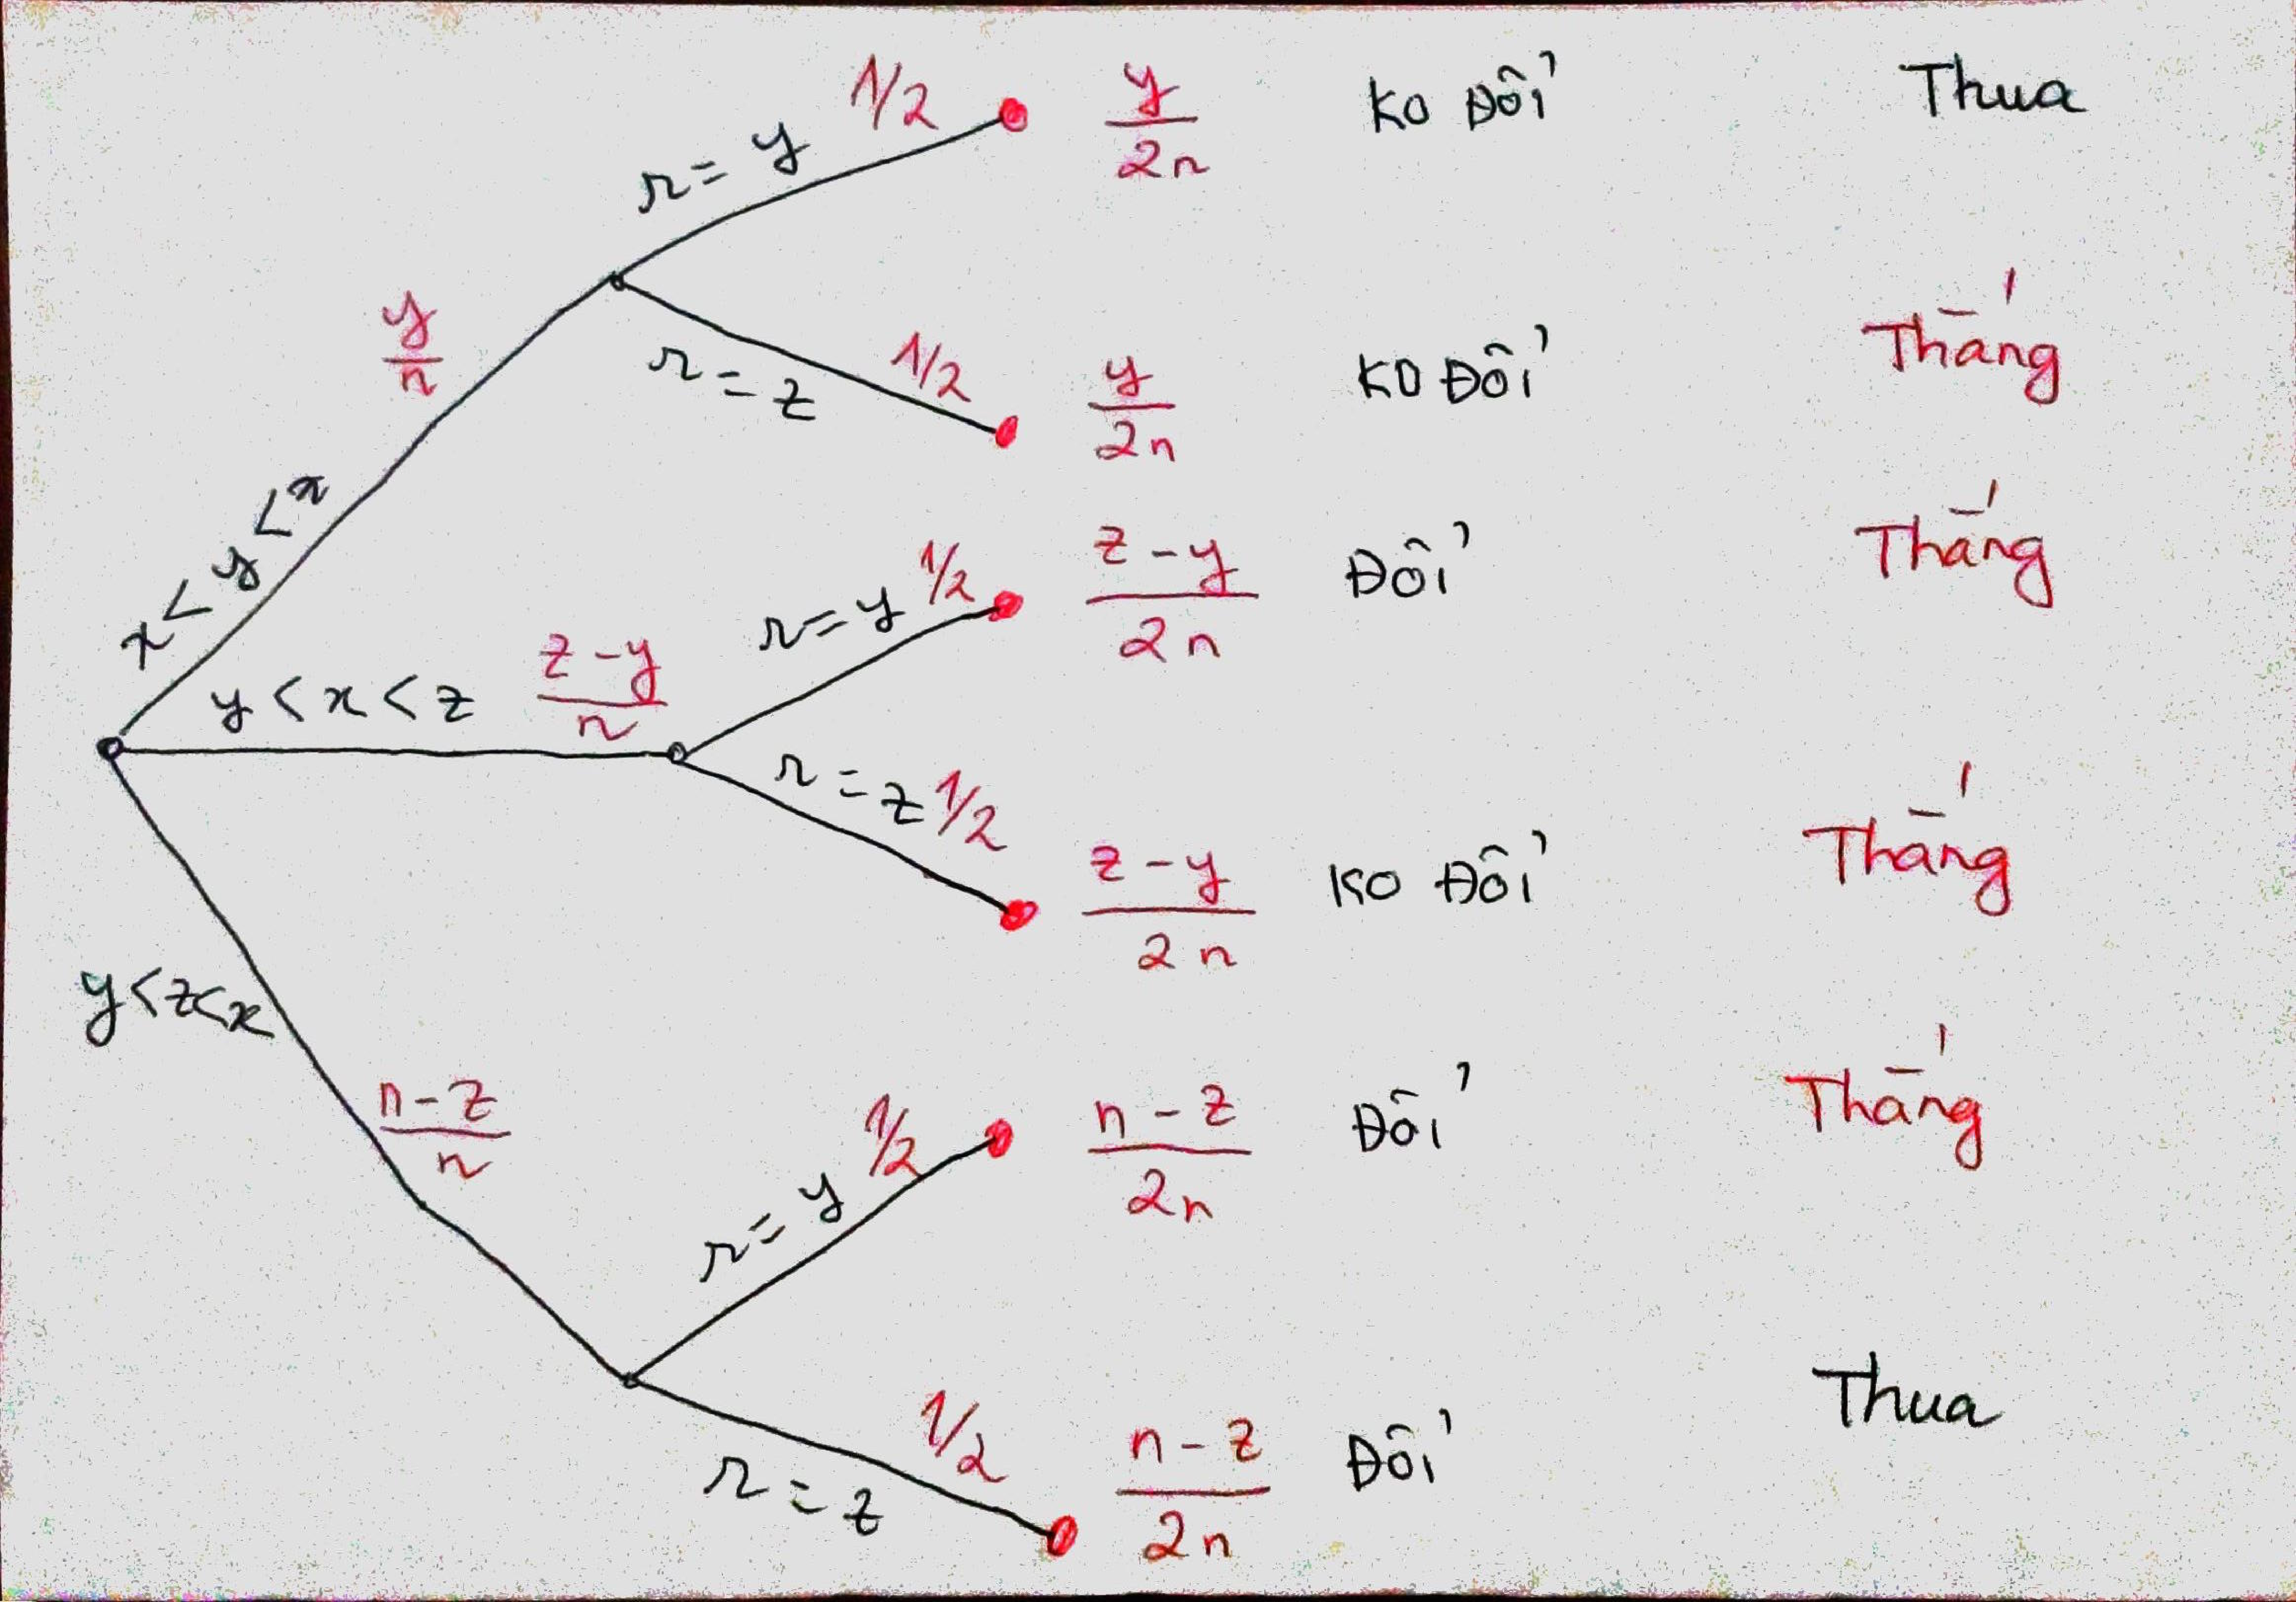
\includegraphics[width=\textwidth]{tree.pdf}			
	\end{center}
\end{frame}
%--- Next Frame ---%

\begin{frame}
	\begin{align*}
		\pr[\text{ thắng }] &= \frac{y}{2n}+\frac{z-y}{2n}+\frac{z-y}{2n}+\frac{n-z}{2n}\\ 
			                &= \frac{n+z - y}{2n}\\
							&= \frac{1}{2}+\frac{z-y}{2n}\\
							&\geq \frac{1}{2}+\frac{1}{2n}
	\end{align*}
\end{frame}

\begin{frame}{Phân bố nhị thức}
	\begin{dfntn}
		\begin{itemize}
			\item Phân bố nhị thức đều 
				\[
					f_n(k) = \binom{n}{k} 2^{-n}\qquad\text{ với } n\geq 1, 0 \leq k\leq n 
				\]
			\item Phân bố nhị thức tổng quát 
			\[
				f_{n,p}(k) = \binom{n}{k} p^k (1-p)^{n-k} 
			\]
		\end{itemize}
	\end{dfntn}
\end{frame}

\begin{frame}
	\begin{block}{}
	\begin{figure}[h] 
	  \centering
	    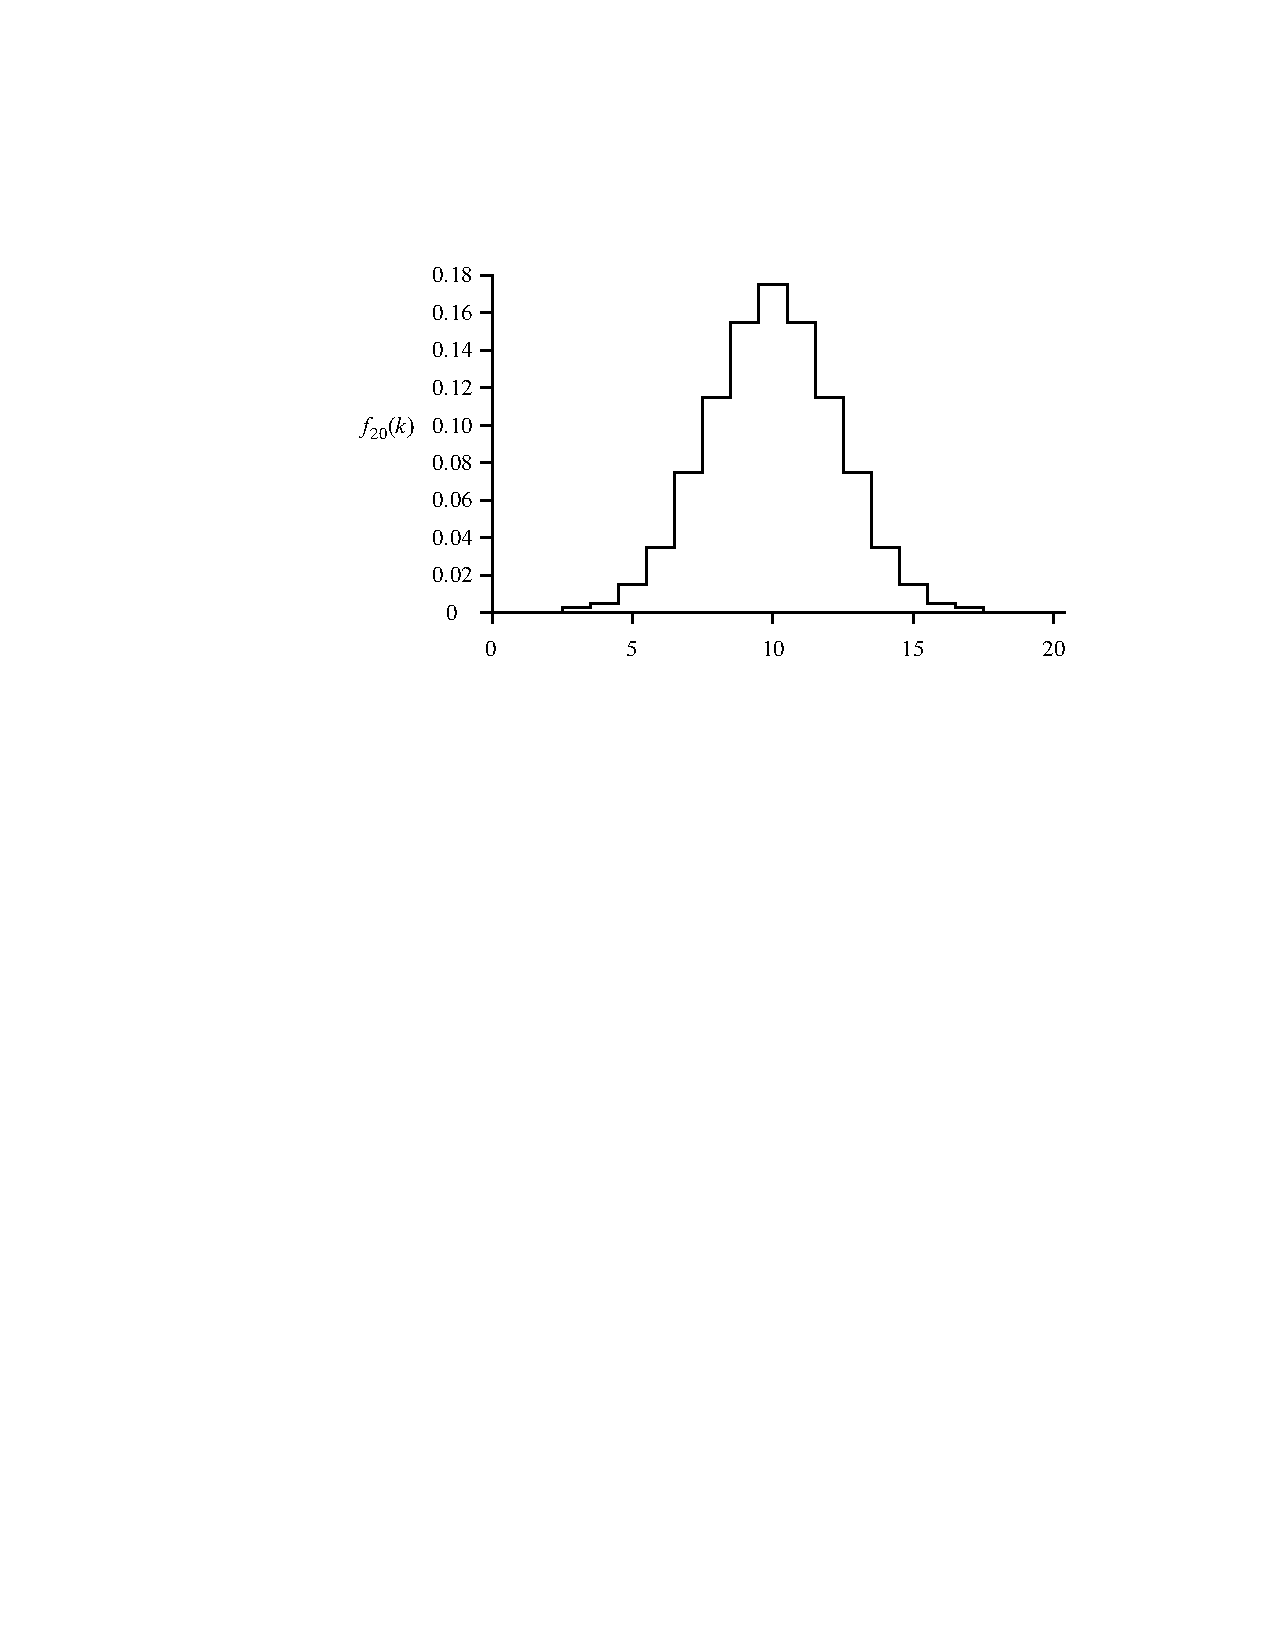
\includegraphics[width=.9\textwidth]{fig184.pdf}
	  \caption{Phân phối nhị thức đều với $n=20$}
	  
	\end{figure}		
	\end{block}
	
\end{frame}

\begin{frame}
	\begin{block}{}
	\begin{figure}[h]
	  \centering
	    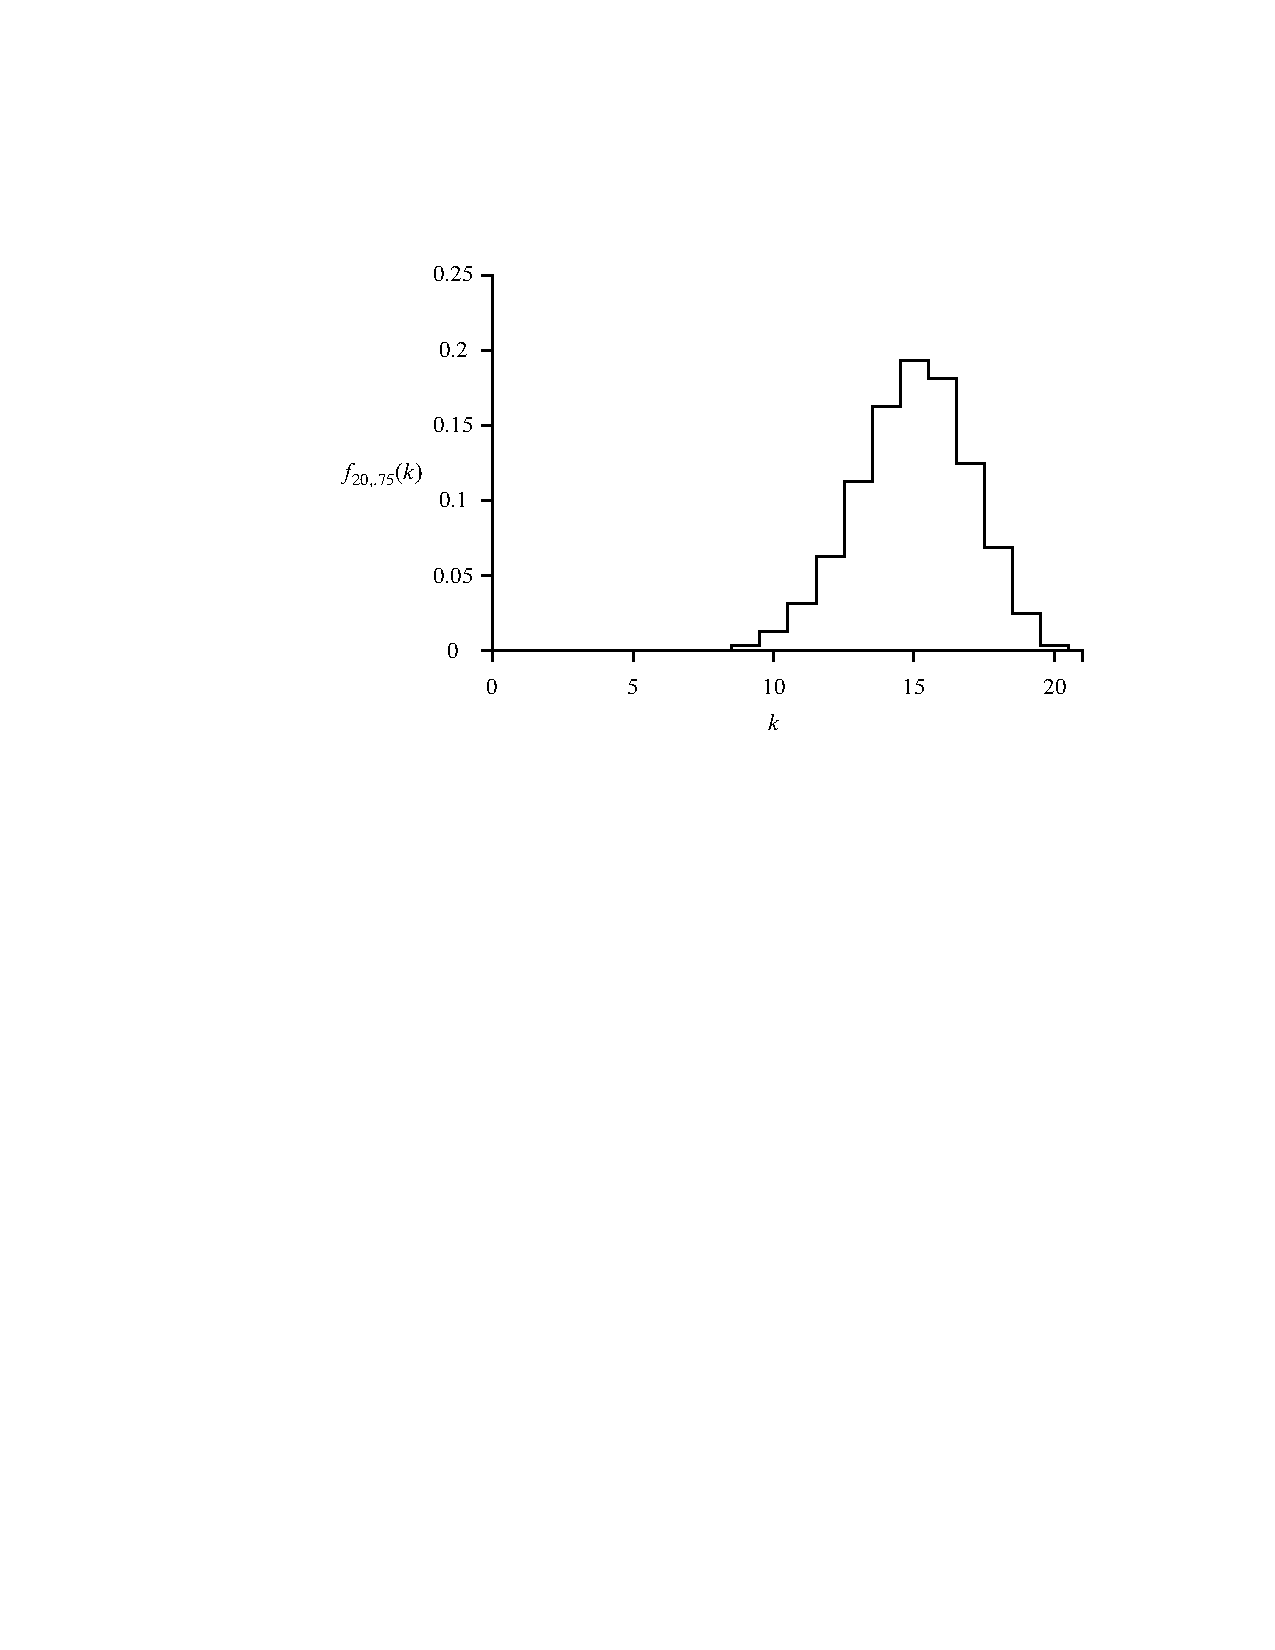
\includegraphics[width=.9\textwidth]{fig185.pdf}
	  \caption{Phân phối nhị thức tổng quát với $n=20$ và $p=0.75$}
	  \label{fig:fig185}
	\end{figure}		
	\end{block}
	
\end{frame}
%--- Next Frame ---%
\begin{frame}{Phân bố nhị thức đều}
	\begin{qstn}
		Hãy tính xác suất nhận được đúng $25$ lần mặt sấp khi tung đồng xu $100$ lần.
	\end{qstn}
\end{frame}
%--- Next Frame ---%
%--- Next Frame ---%
\begin{frame}{Phân bố nhị thức tổng quát}
	\begin{itemize}
		\item Xét một hệ thống với $n$ thành phần $c_1, c_2, \dots, c_n$, mỗi thành phần có thể có lỗi một cách độc lập với xác suất $p$.
		\item Xét $R$ là biến ngẫu nhiên xác định  bởi 
		\[
			R(c_1, c_2, \dots, c_n) = \text{ tổng số lỗi của các thành phần  }
		\]   
	\end{itemize}
	
	\begin{thrm}
		\[
			\pr[R = k] = f_{n,p} (k) = \binom{n}{k} p^k (1-p)^{n-k}. 
		\]
	\end{thrm}
\end{frame}
%--- Next Frame ---%
\end{document}



%%% Local Variables:
%%% mode: latex
%%% TeX-master: t
%%% End:
